\documentclass[11pt]{article}

% Workshop draft. To submit, swap this preamble for the venue's style file.
\usepackage[margin=1in]{geometry}
\usepackage[T1]{fontenc}
\usepackage{lmodern}
\usepackage{microtype}
\usepackage{amsmath,amssymb,amsthm}
\newtheorem{proposition}{Proposition}
\usepackage{graphicx}
\usepackage{booktabs}
\usepackage{xcolor}
\usepackage[font=small,labelfont=bf]{caption}
\usepackage[round,authoryear]{natbib}
\usepackage[colorlinks=true,linkcolor=blue!50!black,citecolor=blue!50!black,urlcolor=blue!50!black]{hyperref}

\newcommand{\hp}{h'}
\newcommand{\ep}{\varepsilon'}
\newcommand{\LO}{\mathrm{LO}}
\newcommand{\todo}[1]{\textcolor{red}{[TODO: #1]}}

\title{Induction Heads as Miscalibrated Bayesian Filters:\\ Recency versus Frequency under Switches and Typos}
\author{Nirbhay Sharma \qquad Gathik Jindal\\
\small \todo{affiliation, emails}}
\date{Draft, 6 October 2026}

\begin{document}
\maketitle

\begin{abstract}
When a context contains a continuation seen often but long ago and a conflicting continuation seen rarely but recently, which one should an induction head copy? We study this in a controlled key--value task in which each key's value occasionally \emph{switches} (rate $h$) and each copy is occasionally a \emph{typo} (rate $\varepsilon$), so that recency is right in one regime and frequency in the other. We derive the Bayes-optimal rule, whose decision boundary depends on the gap since the old copies only logarithmically and not at all on how many old copies there were. Training 218 small transformers, we find that in pure regimes they match the Bayes rule, but when switches and typos are mixed their decisions are best described as the \emph{Bayes rule evaluated at the wrong parameters} (for structured typos; with uniformly random typos a discounted counter fits better): the models act as if values change 3--14$\times$ more often than they do and pull typo rates toward the middle. The miscalibration is lawful, $\hp \approx 1.45\,h^{0.74}$ and $\operatorname{logit}\ep \approx -0.35 + 0.44\operatorname{logit}\varepsilon$, and these laws predict the behaviour of models trained on a held-out setting from its $(h,\varepsilon)$ alone ($R^2 = 0. Frozen and tested on 63 further models, the laws predict new settings inside the fitted range ($R^2 = 0.89$--$0.94$) and transfer unchanged across context length, vocabulary size, number of keys and key frequencies. They extrapolate less well, mainly because a single output scale does not hold at the edges. RoPE models follow the same Bayes form with their own, nearly calibrated, constants.87$). Mechanistically, the decision is made by late attention heads that act as distance-discounted counters; rescaling their ALiBi slopes moves the effective switch rate ($\hp \propto s^{k}$, $k \approx 1.1$--$1.3$), and the trained slopes sit at the minimum of ordinary-data loss, so the miscalibration is loss-optimal for these heads rather than a failure of training. The main claims were tested with pre-registered predictions, null models and replication across positional encodings, depth, width, training length, seeds and hyperparameters; we also report the mechanistic predictions that failed.
\end{abstract}

\section{Introduction}

Induction heads complete a pattern $[A][B]\dots[A] \to [B]$ by attending to the token that followed an earlier occurrence of the current token and copying it \citep{elhage2021mathematical,olsson2022context}. Real contexts often contain \emph{conflicting} earlier occurrences: a name spelled ``Potter'' five times early in a document and ``Potyer'' once near the end. Copying the frequent continuation is right if the recent one is a typo; copying the recent one is right if the value really changed. Neither recency nor frequency is correct in general: which one is optimal depends on how the data were generated.

We make this precise with a key--value task with two noise sources, \emph{switches} (a key's hidden value is redrawn with probability $h$ per step) and \emph{typos} (an observed copy is corrupted with probability $\varepsilon$). The task has an exact Bayes-optimal predictor, so every model can be compared with the best possible rule, and a closed-form decision boundary (Proposition~\ref{prop:bayes}). A simple model of an induction head as a softmax over earlier matches with a distance penalty gives a second, qualitatively different rule: a \emph{discounted counter} (Proposition~\ref{prop:counter}). The two rules disagree in testable ways: the counter counts old copies and decays with distance linearly in the attention score, while the Bayes rule ignores old copies beyond the second and depends on the gap only through $\log G$.

\paragraph{Contributions.}
\begin{itemize}
\item A controlled task and an exact oracle for the recency--frequency trade-off, with a closed-form Bayes decision boundary verified numerically (Section~\ref{sec:setup}).
\item A behavioural finding: across 218 trained models, conflict decisions are described best by the Bayes rule at \emph{miscalibrated} parameters $(\hp,\ep)$, not by a counter. The description generalises to unseen probe layouts and is not a generic property of smooth curves or of sums of counters (Section~\ref{sec:behaviour}).
\item Laws of miscalibration with confidence intervals that predict a held-out training setting's models from its $(h,\varepsilon)$ alone, tested before training on 63 new models in new settings, context lengths, vocabularies, numbers of keys and positional encodings (Section~\ref{sec:laws}).
\item A causal account of the miscalibration: the late heads' fading rates set $\hp$, and the trained rates minimise ordinary-data loss (Section~\ref{sec:causal}).
\item A partial mechanism, together with the mechanistic predictions that failed (Section~\ref{sec:mechanism}).
\end{itemize}

\section{Setup}
\label{sec:setup}

\begin{figure}[t]
\centering
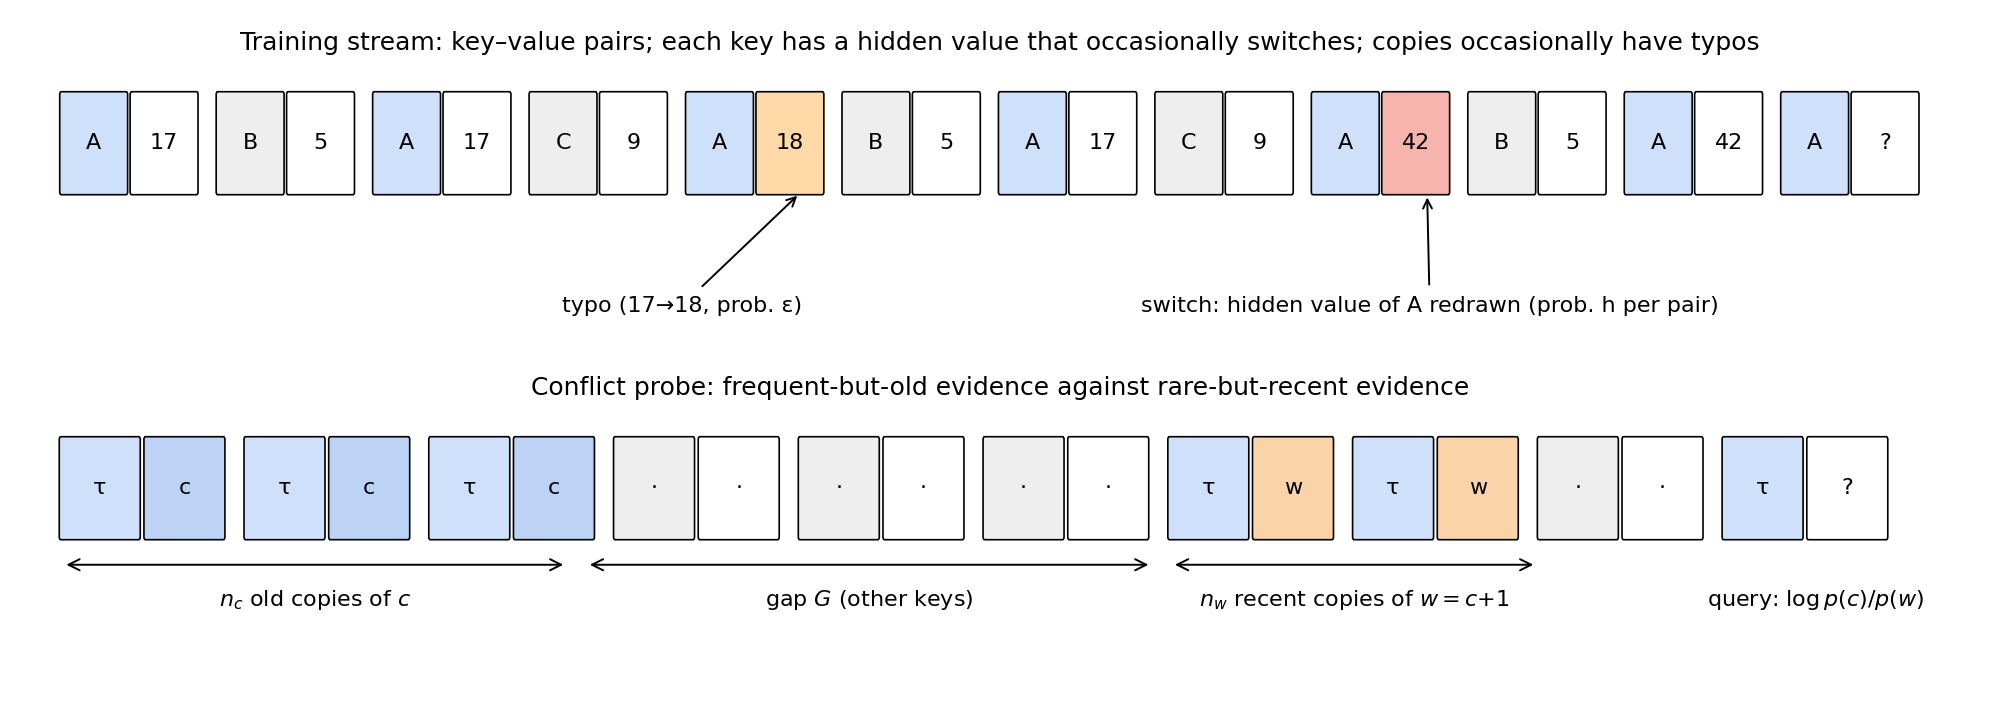
\includegraphics[width=\linewidth]{figures/fig_task.png}
\caption{\textbf{Task and probes.} Top: training sequences are key--value pairs; each key has a hidden value that is redrawn with probability $h$ per pair (switch), and each observed value is a typo $z{+}1$ with probability $\varepsilon$. Bottom: a conflict probe places $n_c$ old copies of $c$, a gap of $G$ pairs, and $n_w$ recent copies of $w = c{+}1$ before the query.}
\label{fig:task}
\end{figure}

\paragraph{Task.} A sequence is $\texttt{BOS}, k_1, y_1, \dots, k_N, y_N$ with $N = 256$ pairs, $K = 16$ keys drawn from a Zipf distribution (identities permuted per sequence) and $V = 64$ values. Each key $k$ has a hidden value $z_k(t)$, uniform at $t=0$ and independently redrawn uniformly with probability $h$ per pair. The observed value is $y_t = z_{k_t}(t)$ with probability $1-\varepsilon$ and the typo $z_{k_t}(t){+}1 \bmod V$ otherwise. The loss is next-token cross-entropy on value positions only. Fresh data are generated at every step.

\paragraph{Bayes oracle.} Keys are independent hidden Markov models: between two sightings of a key $g$ pairs apart, the value survives with probability $s=(1-h)^g$ and is otherwise uniform. An exact forward filter gives $p^*(y_t \mid \text{history})$ at every position. We verified it against brute-force enumeration and an independent re-implementation, and checked its calibration on generator samples (expected calibration error $< 0.01$).

\paragraph{Probes.} A probe (Figure~\ref{fig:task}, bottom) uses a key $\tau$ absent from the background: $n_c \in \{1,2,4,8\}$ copies of $c$, a gap of $G \in \{2,\dots,128\}$ pairs, $n_w \in \{1,\dots,4\}$ copies of $w = c{+}1$, all 4 pairs apart, and a query 4 pairs after the last $w$. We record the log-odds $\LO = \log p(c)/p(w)$ of the model and of the oracle, averaged over 256 random backgrounds per cell (112 cells).

\begin{proposition}[Bayes boundary]\label{prop:bayes}
For the probe above with structured typos, the two dominant hypotheses are ``no switch in the gap, the $w$'s are typos'' and ``a switch to $w$ in the gap, the $w$'s are clean''. With $s = (1-h)^G$,
\[
\log\frac{P(z=c)}{P(z=w)} \approx \log\frac{s}{1-s} - n_w\log\frac{1-\varepsilon}{\varepsilon} + \log V,
\]
so the Bayes rule switches to the recent value iff $\frac{s}{1-s} < \frac{1}{V}\left(\frac{1-\varepsilon}{\varepsilon}\right)^{n_w}$, which for small $hG$ reads
$\log(hG) > \log V - n_w \log\frac{1-\varepsilon}{\varepsilon}$.
\end{proposition}

The boundary is independent of $n_c$ once $n_c \ge 2$ (old copies are explained equally well under both hypotheses), depends on the gap through $\log G$, and each additional recent copy shifts $\log G^*$ by $\log\frac{1-\varepsilon}{\varepsilon}$. Against the exact oracle, the formula's switch-over gap is within a median 10--15\% for $hG^* \le 3$; going from 2 to 16 old copies changes the exact log-odds by at most 0.11 nats; and the per-copy shift is exact to within 2\% for $hG^* \le 0.3$ (it is up to 55\% smaller when $hG^* \approx 1$--3).

\begin{proposition}[Discounted counter]\label{prop:counter}
If an attention head's logit on an earlier copy $j$ is $\beta m_j - \lambda d_j$ (match quality $m_j$, distance $d_j$), non-matching positions receive negligible attention, and the OV circuit copies the value with a common gain $\gamma$, then the head's contribution to the value logits is $\gamma A(v)/Z$ with $A(v) = \sum_{j:\, y_j = v} e^{\beta m_j - \lambda d_j}$. With clustered copies it prefers $c$ iff $\log(n_c/n_w) > \lambda(d_c - d_w)$.
\end{proposition}

\noindent A sum of such heads with positive gains is strictly increasing in $n_c$, unlike the Bayes rule.

\paragraph{Models and training.} Pre-LayerNorm transformers of width 128 with 4 heads: 2-layer attention-only (L2), 2-layer with MLPs (L2+MLP) and 3-layer attention-only (L3), with a learnable ALiBi slope per head \citep{press2022alibi}, RoPE \citep{su2024roformer} or learned absolute positions. AdamW, learning rate $10^{-3}$ with warmup and cosine decay, batch 128, 20k steps, bf16. A clean-data gate ($h=\varepsilon=0$) reaches 100\% accuracy on repeat sightings and the Bayes loss to within $10^{-4}$ nats. We trained 218 models: 2 gate models, 36 in four corner and mixed settings, 69 for positional-encoding controls, conflict-enriched training, a uniform-typo corner and a $3\times4$ grid $h \in \{0.003, 0.01, 0.03\}$, $\varepsilon \in \{0.05, 0.1, 0.2, 0.3\}$, 16 longer or wider models, 32 audit runs (reproducibility, learning rate, batch size), and 63 runs testing the frozen laws (Section~\ref{sec:laws}): new $(h,\varepsilon)$, context lengths 192 and 512, $V \in \{32, 128\}$, $K \in \{8, 32\}$, uniform key frequencies and uniform typos, and RoPE on the full grid. Models without positional encoding did not train within the budget.

\section{Models follow the Bayes shape at the wrong parameters}
\label{sec:behaviour}

\begin{figure}[t]
\centering
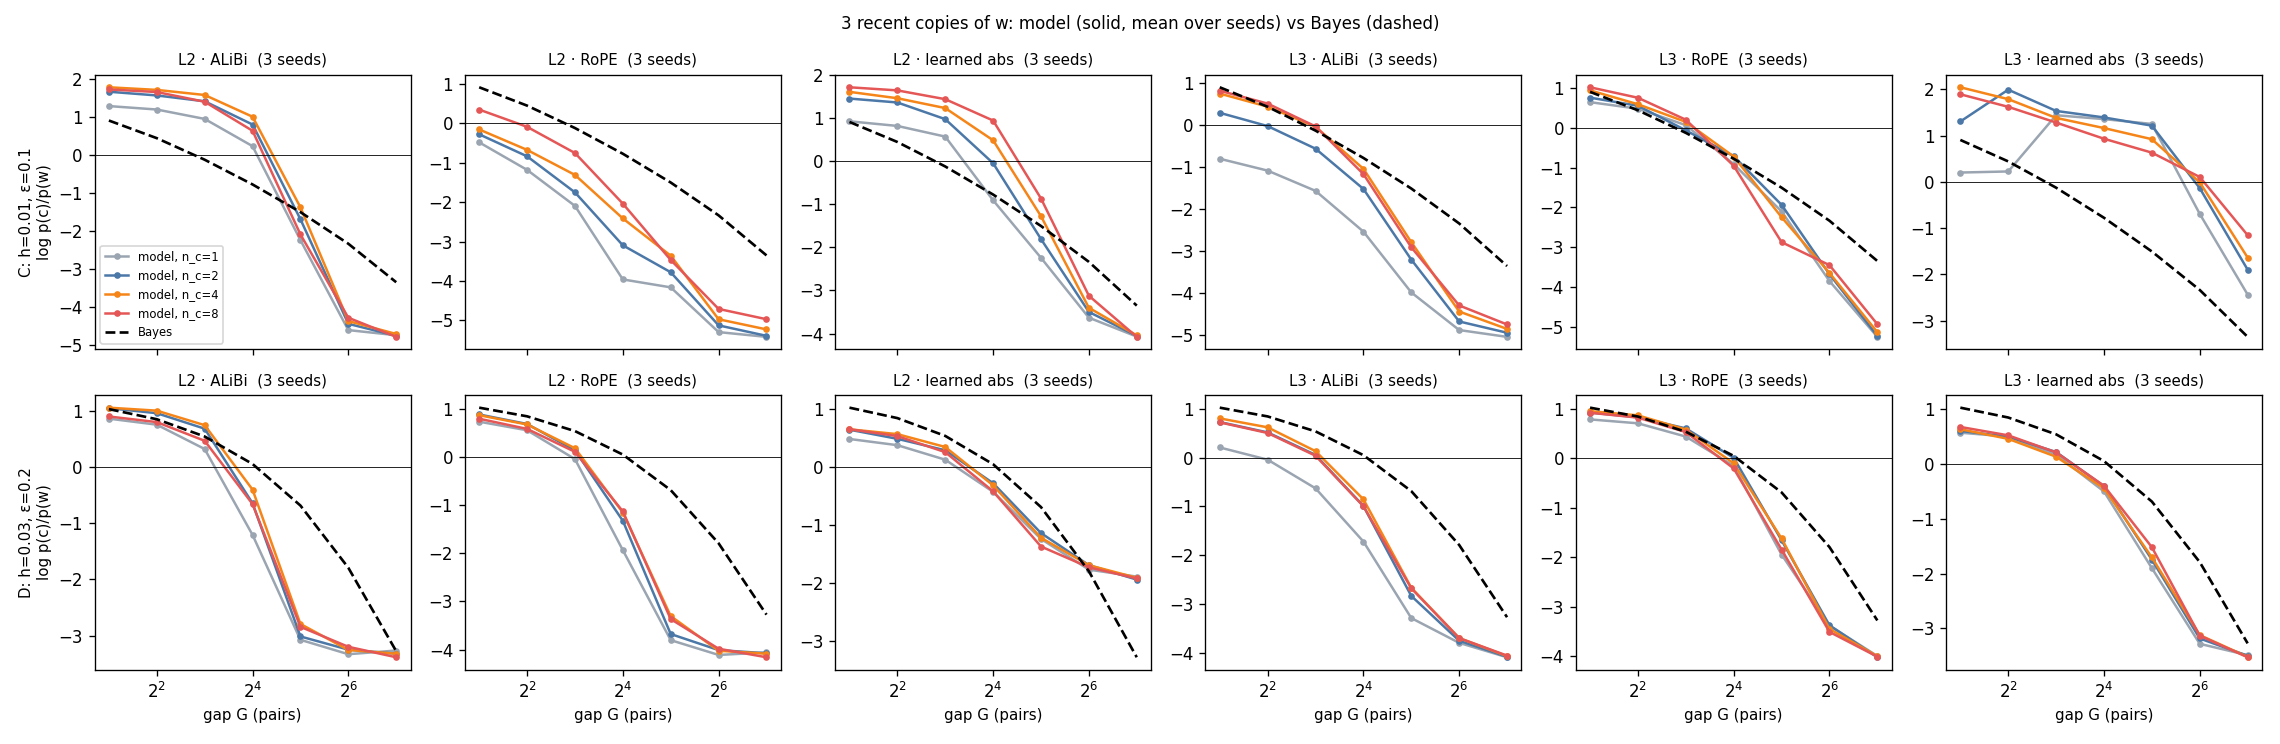
\includegraphics[width=\linewidth]{figures/pe_control_nw3.png}
\caption{\textbf{Conflict behaviour vs.\ Bayes.} Log-odds for 3 recent copies against the gap, at $(h,\varepsilon) = (0.01, 0.1)$ (top) and $(0.03, 0.2)$ (bottom), for six architectures (mean of 3 seeds; colours $n_c = 1,2,4,8$; dashed: Bayes). Models hold on to the old value and then switch more abruptly than Bayes, ending far more confident in $w$.}
\label{fig:curves}
\end{figure}

\paragraph{Pure regimes match Bayes.} With switches only ($\varepsilon=0$) or typos only ($h=0$), every model agrees with the Bayes decision on 90--100\% of probes. With uniform typos and no switches, where counting is optimal, models count: a second old copy raises the log-odds by $+2.34$ (Bayes $+2.59$).

\paragraph{Mixed regimes do not.} When switches and typos are mixed, models switch from the old to the recent value more abruptly than Bayes (Figure~\ref{fig:curves}). The steepest drop in log-odds per doubling of the gap is $1.2$--$11.5\times$ the Bayes value in all 12 grid settings (median $3.5\times$). The effect is strongest with ALiBi but persists with RoPE and learned positions (1.15--2.4$\times$ in 11 of 12 encoding--depth--setting combinations).

\paragraph{Which rule?} For each model we fitted five descriptions to its 112 probe log-odds and scored them on held-out gaps: the Bayes rule at the true $(h,\varepsilon)$ with a fitted scale and offset; the Bayes rule at fitted $(\hp,\ep)$ (4 parameters); the discounted counter of Proposition~\ref{prop:counter} with an exponential or power-law kernel (5 parameters); and an unnormalised evidence sum (5 parameters). Bayes at fitted parameters is the best held-out description for 75 of 84 mixed-regime models (median held-out $R^2$ 0.85--0.95 per architecture, against 0.37--0.74 for the counter; Figure~\ref{fig:fits}a) and for 24 of 24 models in the learning-rate and batch-size sweep. The fits are stable: a second optimiser on a finer grid recovers the same $\hp$ in 99\% of models, and bootstrap 90\% intervals span a factor of 1.30 ($\hp$) and 1.14 ($\ep$).

\begin{figure}[t]
\centering
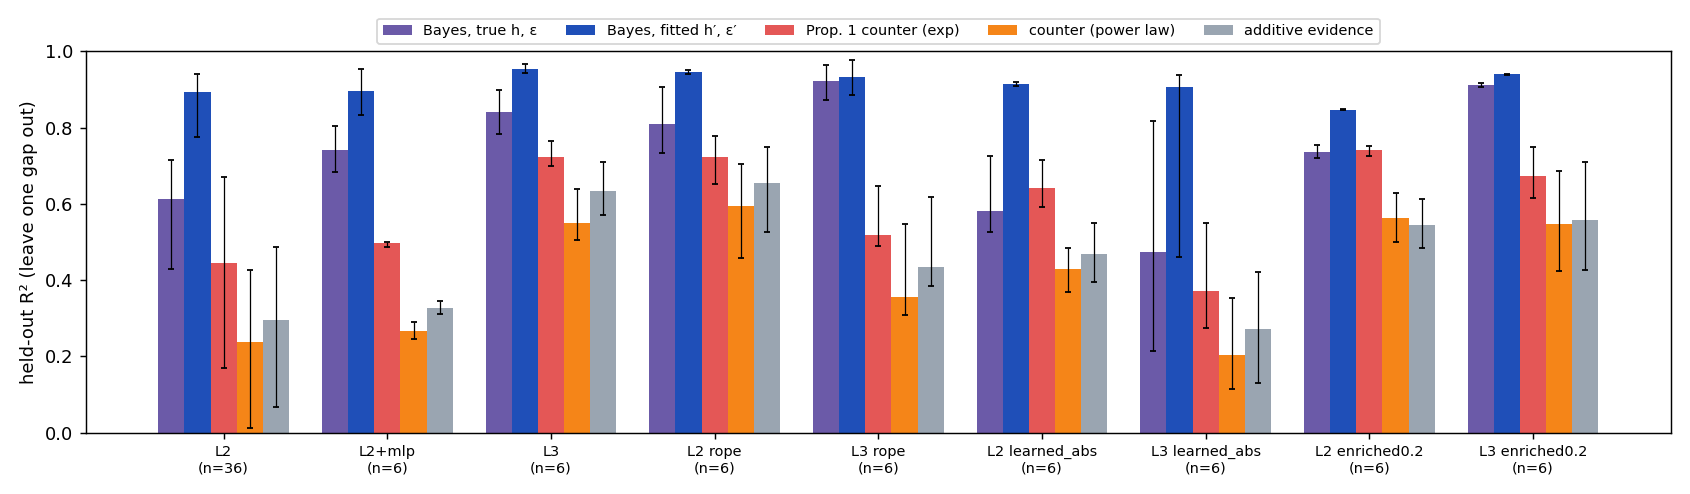
\includegraphics[width=\linewidth]{figures/fit_quality.png}\\[2pt]
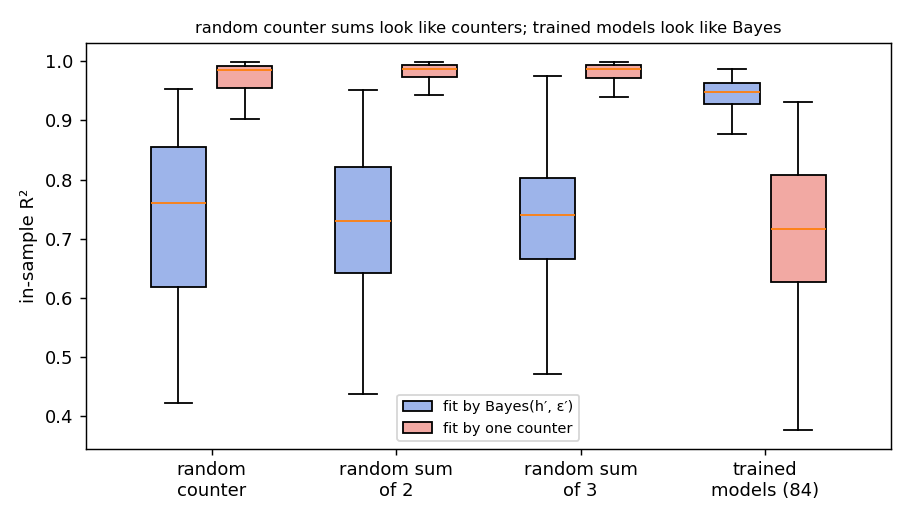
\includegraphics[width=0.62\linewidth]{figures/run3_bridge.png}
\caption{\textbf{(a) Top:} held-out $R^2$ of five descriptions by architecture (median, IQR). \textbf{(b) Bottom:} random counters and random sums of 2--3 counters are fit by a single counter ($R^2 \approx 0.99$) and only moderately by Bayes at fitted parameters ($\approx 0.74$); trained models show the opposite.}
\label{fig:fits}
\end{figure}

\paragraph{Generalisation.} Fitted on the original probe layout only, Bayes$(\hp,\ep)$ predicts probes with copies 2 or 8 pairs apart at $R^2 = 0.93$ and beats the best counter in 90\% of 168 model--layout pairs; refitting on the new layouts returns $(\hp,\ep)$ within $2\times$ in 97\% of cases. In a swapped layout where the old copies are the typo-variants of the recent value, the Bayes rule always picks the recent value; the models do too, against 8 old copies at short gaps, while every fitted counter predicts the opposite (lower error than the best counter in 94\% of models).

\paragraph{Not a generic fit.} The Bayes family is not a universal fitter of smooth curves: on random smooth monotone surfaces it reaches median $R^2 = 0.73$, on cell-shuffled model surfaces 0.07, and on random sums of counters 0.74, against 0.95 on the trained models (Figure~\ref{fig:fits}b).

\section{Laws of miscalibration}
\label{sec:laws}

\begin{figure}[t]
\centering
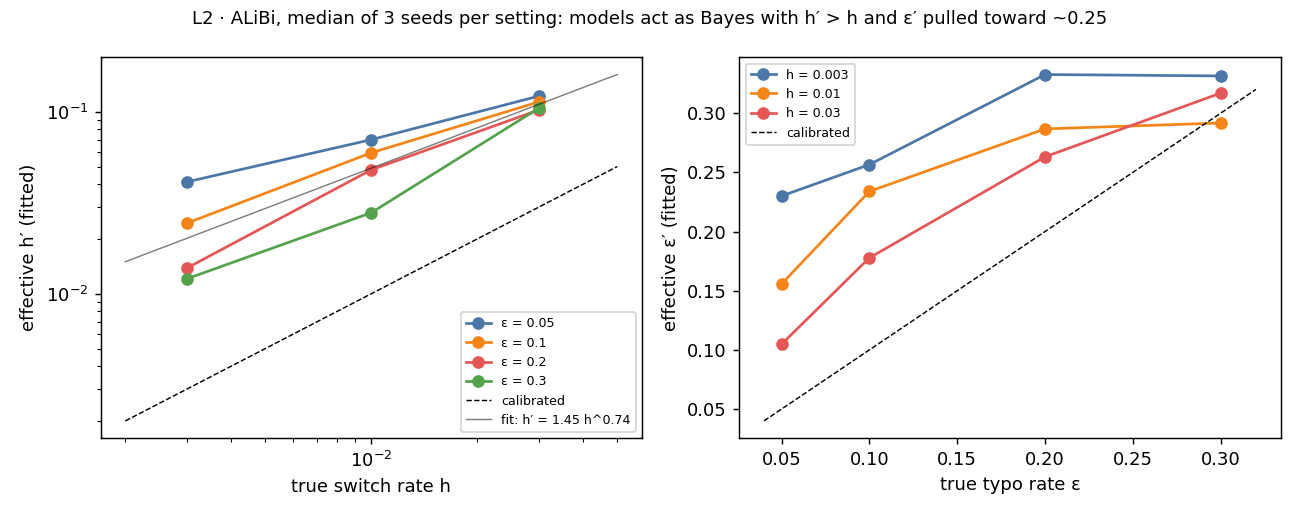
\includegraphics[width=0.85\linewidth]{figures/effective_params.png}
\caption{\textbf{Effective parameters vs.\ true ones} (L2, ALiBi; median of 3 seeds per setting). Models always overestimate the switch rate and compress the typo rate toward the middle.}
\label{fig:laws}
\end{figure}

On the 12-setting grid (2-layer ALiBi models), the fitted parameters follow simple laws (Figure~\ref{fig:laws}; point estimates from the 12 setting medians, 95\% intervals from resampling seeds):
\begin{equation}
\hp = 1.45\,[1.29, 1.78]\cdot h^{\,0.74\,[0.71,\,0.78]},\qquad
\operatorname{logit}\ep = -0.35\,[-0.47, -0.04] + 0.44\,[0.35, 0.57]\cdot\operatorname{logit}\varepsilon .
\label{eq:laws}
\end{equation}
$\hp$ exceeds $h$ by $2.8$--$14\times$ (significantly in 92\% of models), most when switches are rare, and the typo rate is pulled toward $\approx 0.25$--$0.35$. Measured on the same probes, each recent copy carries a median $0.46\times$ (range $0.24$--$1.06$) of its exact Bayes evidence, with the shortfall largest when typos are rare.

\paragraph{Prediction from data statistics.} To test whether Eq.~\eqref{eq:laws} is predictive rather than descriptive, we fitted it on 11 of the 12 settings and predicted the probe behaviour of the models trained on the 12th from its $(h,\varepsilon)$ alone. The prediction reaches median $R^2 = 0.87$ over held-out models, above the true Bayes rule even with scale and offset fitted on the held-out models themselves (0.74), the mean surface (0.55) and an average counter (0.25). The weakest held-out settings are $(0.003, 0.3)$ at 0.57 and $(0.03, 0.05)$ at 0.72.

\paragraph{Stress tests.} Three further checks bound how far Eq.~\eqref{eq:laws} can be trusted.
\begin{itemize}
\item \emph{Extrapolation.} Holding out a whole level of $h$ or $\varepsilon$ and predicting it from the rest gives median $R^2 \ge 0.78$ for 6 of 7 levels. The exception is predicting $h = 0.03$ from the two lower levels, at 0.72.
\item \emph{Noise ceiling.} The mean surface of the other seeds predicts a model's surface at $R^2 = 0.98$, which bounds any description. Each model's own fitted Bayes rule reaches 0.94, and the law reaches 0.87 on held-out settings, about 89\% of the ceiling. Its sign agrees with the model's decision on 95\% of the probes that have a clear preference.
\item \emph{Separability.} $\hp$ also depends on $\varepsilon$: at $h = 0.003$ it varies $3.4\times$ across typo rates, and $2.9\times$ when $\ep$ is held at the law's value. So the dependence is real and not the trade-off between the two fitted parameters. As a description of the parameters, the separable law explains 80\% of the variance of $\log\hp$ and 68\% of $\operatorname{logit}\ep$ across settings. Adding cross terms does not improve held-out prediction of behaviour ($R^2$ 0.85 vs.\ 0.87).
\end{itemize}

\begin{figure}[t]
\centering
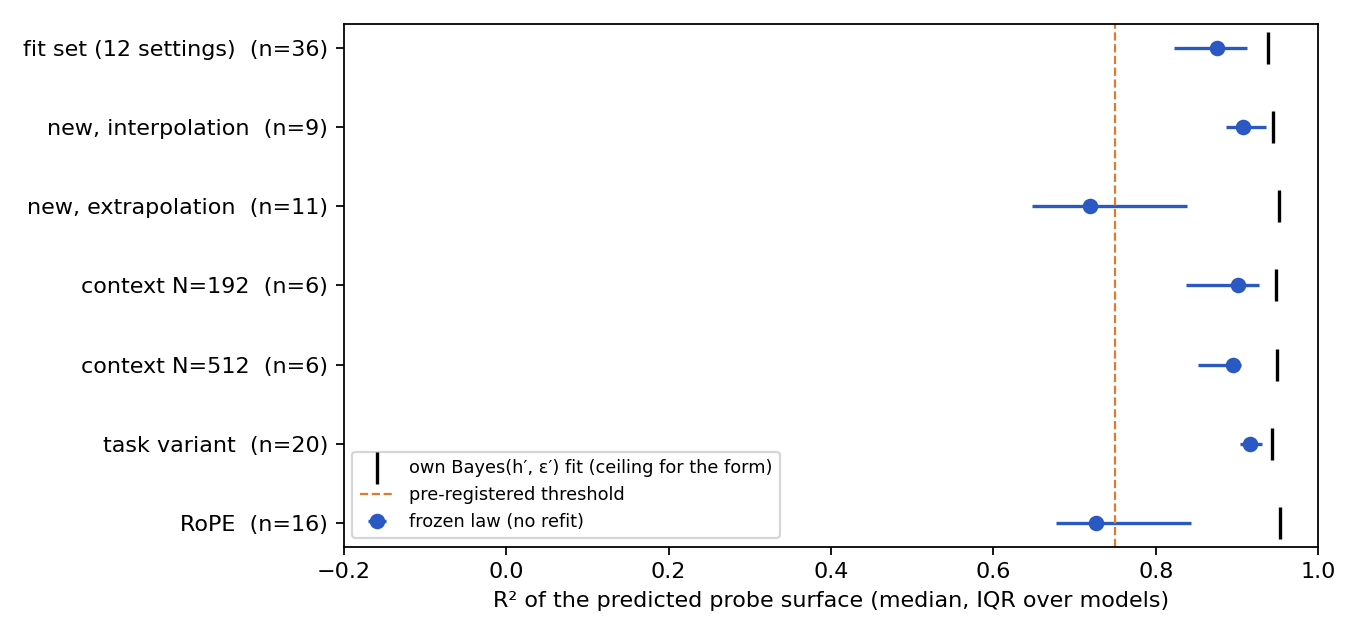
\includegraphics[width=0.85\linewidth]{figures/scope_r2.png}
\caption{\textbf{The frozen law on 63 models trained after it was fixed} (run 6). Points: median $R^2$ of the predicted probe surface (bars: IQR over models); ticks: each model's own Bayes$(\hp,\ep)$ fit, the ceiling for the functional form. Task variants: $V \in \{32, 128\}$, $K \in \{8, 32\}$, uniform keys, uniform typos. The RoPE row applies the ALiBi constants, which do not transfer; RoPE's own constants reach 0.89 on held-out settings.}
\label{fig:scope}
\end{figure}

\paragraph{New settings (pre-registered).} We froze Eq.~\eqref{eq:laws} (with median scale and offset) and trained 21 new models (Figure~\ref{fig:scope}) at seven $(h,\varepsilon)$ settings that had not been used to fit it.
\begin{itemize}
\item \emph{Inside the fitted range}, at $(0.005, 0.07)$, $(0.02, 0.15)$ and $(0.007, 0.25)$, the law predicts the new models' probe surfaces at median $R^2 = 0.89$--$0.94$, with $\hp$ within a factor of 1.7.
\item \emph{Outside it}, the law holds at $\varepsilon = 0.02$ ($R^2 = 0.88$) and narrowly misses at $h = 0.001$ and $h = 0.06$ (0.72, 0.73). It fails at $\varepsilon = 0.4$, where the models' surfaces are nearly flat: the absolute error there (0.71 nats) matches that on the fitted grid (0.68), but the variance is tiny.
\end{itemize}
Over all new models, the median $R^2$ is 0.87, equal to the leave-one-setting-out estimate made before these runs. Bayes at fitted parameters again beats both counters on held-out gaps in all 20 non-flat models.

A post-hoc analysis locates the failures. The predicted beliefs $(\hp, \ep)$ transfer; what does not transfer to the edges is the single output scale $b$, which ranges from 0.87 at $\varepsilon = 0.4$ to 4.8 at $h = 0.001$. There is also a dependence of $\ep$ on $h$: a variant of the law with cross terms, fitted on the original grid only, predicts $h = 0.06$ at $R^2 = 0.93$.

\paragraph{Context length (pre-registered).} We had suspected that the exponent below 1 comes from switch timescales longer than the context. That predicted a lower $\hp$ at small $h$ and a larger exponent with longer contexts. Training at $N = 192$ and $512$ pairs (versus 256) refuted this. At $h = 0.003$, $\hp$ is $1.02\times$ its $N = 256$ value at $N = 512$ (the prediction was $\le 0.77\times$) and $1.17\times$ at $N = 192$. The exponent measured over $h \in \{0.003, 0.01, 0.03\}$ is 0.63, 0.67 and 0.62. The frozen law predicts the models at all three lengths equally well (median $R^2 = 0.90$), so its constants do not depend on context length in this range.

\paragraph{Vocabulary and number of keys (pre-registered).} With the Bayes rule computed for each model's own $V$, the frozen law predicts models trained with $V = 32$ or $128$ values, or $K = 8$ or $32$ keys, at median $R^2 = 0.89$--$0.94$, and their $\hp$ stays within $0.89$--$1.15\times$ that of the default task. Had the models ignored $V$, matching them with the $V$-aware Bayes rule would have required $\hp$ to halve or double. The observed change is about a fifth of that, so the models' switch-over moves with $\log V$ much as the Bayes boundary does.

\paragraph{Key frequencies and typo structure (pre-registered).} With uniform instead of Zipf key frequencies the frozen law still holds ($R^2 = 0.93$ and $0.83$; $\hp$ at $0.92$ and $0.69\times$ the default). With uniformly random typos it does not ($R^2 = 0.17$, $0.34$), which we expected. More importantly, in these models a discounted counter predicts held-out gaps better than the Bayes rule at fitted parameters. This is not an artifact of our fitting range: allowing $\ep$ up to 0.95 (any $\varepsilon < 63/64$ is a valid uniform channel) improves the Bayes fit but leaves the counter better in 4 of 5 uniform-typo models, including the three trained without switches. The Bayes-like behaviour therefore depends on structured typos, where a typo is a recognisable variant of the true value. This is consistent with the content discount of typo-variant copies in Section~\ref{sec:mechanism}, though we have not tested that link directly.

\paragraph{RoPE (pre-registered).} Across the same 12-setting grid, RoPE models are again best described by the Bayes rule at fitted parameters (own-fit $R^2$ 0.93--0.97, better than both counters in every model). They are much closer to calibrated: $\hp/h$ is $1.7$--$4.4$ against $2.8$--$14$ for ALiBi, and lower at all 12 settings. Their typo belief is nearly exact ($\operatorname{logit}\ep = 0.01 + 1.02\operatorname{logit}\varepsilon$, $R^2 = 0.91$). A law with RoPE's own constants predicts held-out settings at median $R^2 = 0.89$, but our pre-registered criterion for the same functional form failed: a power law in $h$ fits RoPE's setting medians with $R^2 = 0.68$ (criterion $\ge 0.8$). Post hoc, this traces to one unidentifiable fit (one seed at $(0.003, 0.3)$; $\hp \approx 0$ with scale 128). Without it, $\hp = 1.26\,h^{0.88}$ with $R^2 = 0.89$. The ALiBi constants do not transfer to RoPE (median $R^2 = 0.73$).

\paragraph{Robustness.} The qualitative pattern holds for every variation tested: retraining with the same seed reproduces $\hp$ within 4\% and $\ep$ within 2\% (probe-surface correlation $\ge 0.9998$); new seeds fall within the original range; learning rates $3\times10^{-4}$ and $3\times10^{-3}$ and batch 256 leave ALiBi models at $\hp/h = 3.3$--$6.3$; three times longer training changes $\hp$ by $\times 0.76$--$1.17$. Width 256 brings $\hp$ closer to $h$, much more for RoPE ($1.3$--$1.5\times$) than for ALiBi ($2.9$--$5.3\times$). Training with 20\% of the loss on extra conflict sequences, whose answers are sampled from the Bayes predictive, roughly halves the excess abruptness of the switch but raises the excess loss on ordinary data two- to four-fold.

\section{The fading rate sets the believed switch rate}
\label{sec:causal}

\begin{figure}[t]
\centering
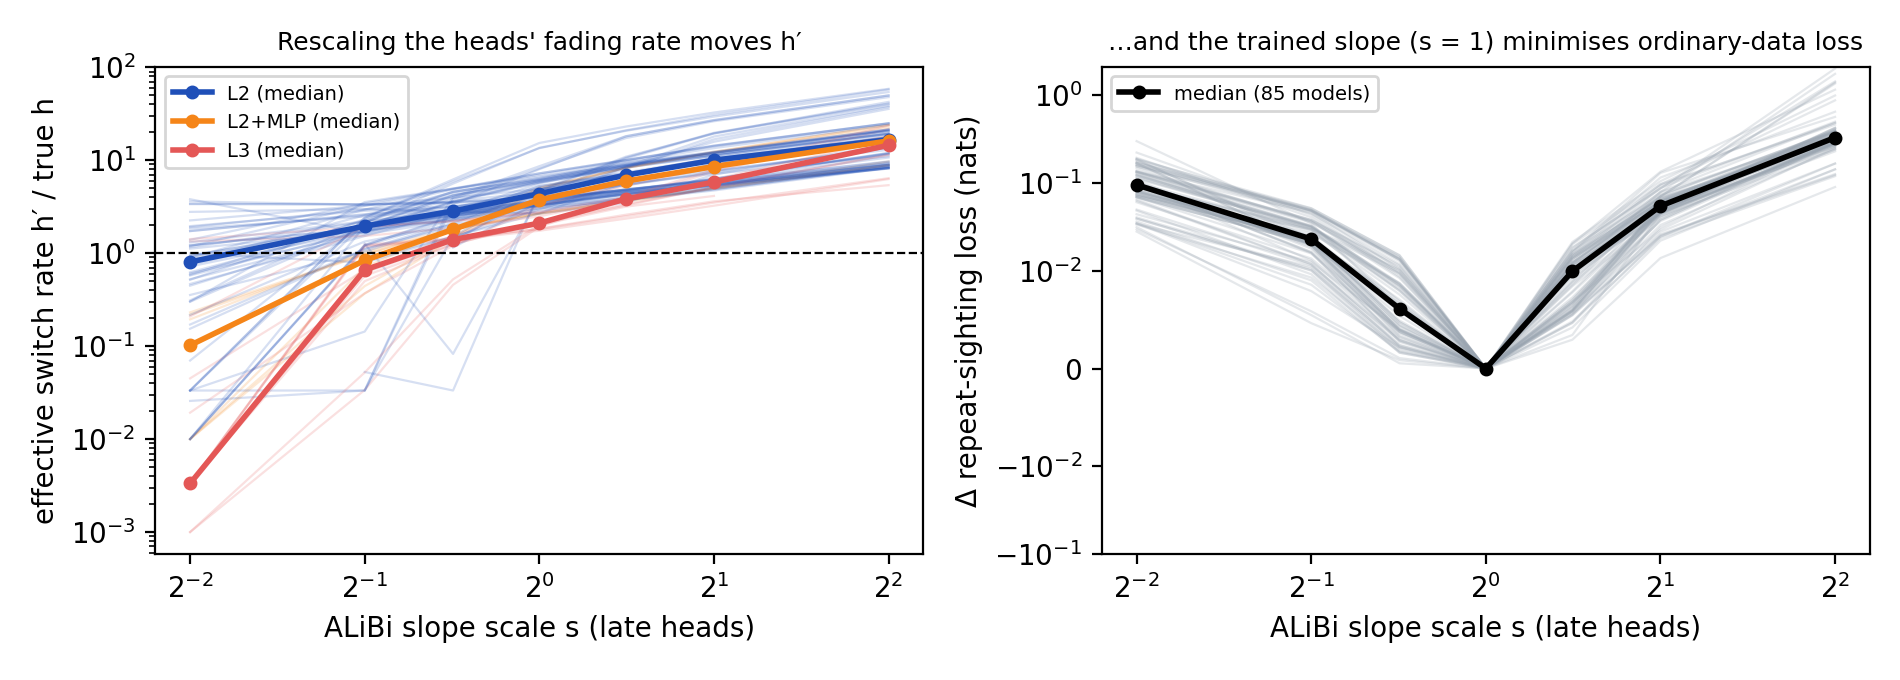
\includegraphics[width=\linewidth]{figures/fig_slope.png}
\caption{\textbf{Slope surgery} on 85 ALiBi models. Left: multiplying the late heads' slopes by $s$ moves the effective switch rate ($\hp \propto s^k$). Right: ordinary-data loss is minimised at the trained slopes.}
\label{fig:slope}
\end{figure}

Multiplying the ALiBi slopes of the late (copy) heads by $\times0.5$ and $\times2$ moves the median $\hp$ from 0.055 to 0.030 and 0.109; $\hp$ is monotone in the scale in 56 of 57 models (the exception is a trade-off along the $\hp$--$\ep$ ridge) and the model-free switch-over gap is monotone in 39 of 39 models where it is finite. Over a finer sweep $s \in [0.25, 4]$, $\log\hp$ is linear in $\log s$ (per-model $R^2 = 0.93$) with elasticity $k = 1.1$--$1.2$ for 2-layer attention-only models (median over all 85 models 1.29, IQR 0.82--2.40; larger for MLP and 3-layer models). Removing all late heads removes the decision (median $-96\%$ in $|\LO|$).

The trained slopes sit at the minimum of ordinary-data loss in all 85 models (Figure~\ref{fig:slope}, right): the loss is flat nearby ($+0.006$ to $+0.010$ nats for $s = 0.71$ and $1.41$), but bringing $\hp$ down to the true $h$ requires $s \approx 0.44$ and costs a median $+0.044$ nats (IQR 0.020--0.082), about three times the models' excess loss over Bayes. In ordinary data, conflicts are common (57--88\% of repeat sightings have a conflicting history, and the Bayes answer differs from ``copy the most recent value'' at 4--14\% of positions), so the miscalibration is not due to a lack of conflicts: for these heads, the fading rate that is best for ordinary prediction implies a too-high switch rate on conflict probes.

\section{Mechanism: what is and is not explained}
\label{sec:mechanism}

\begin{figure}[t]
\centering
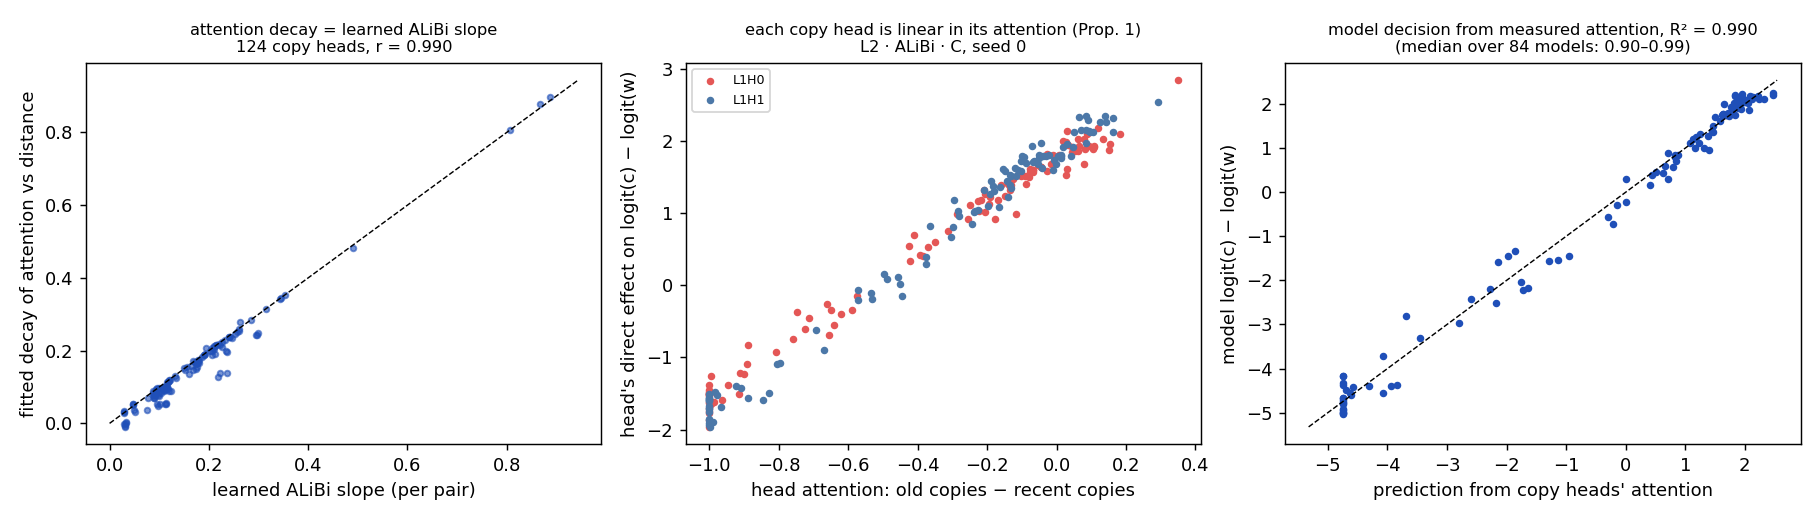
\includegraphics[width=\linewidth]{figures/mechanism.png}
\caption{\textbf{Copy heads as counters.} Left: for 124 ALiBi copy heads, the decay of attention with distance equals the learned slope ($r=0.990$). Middle: each copy head's direct effect on $\operatorname{logit}(c) - \operatorname{logit}(w)$ is linear in its attention to old minus recent copies. Right: the model's decision predicted from measured attention.}
\label{fig:mech}
\end{figure}

An exact decomposition of $\operatorname{logit}(c) - \operatorname{logit}(w)$ at the query into embeddings, heads and MLPs (final LayerNorm linearised at the actual residual; reconstruction error $< 2\times10^{-4}$) shows that 2--3 late heads carry 91--100\% of the decision in attention-only models. Each behaves like Proposition~\ref{prop:counter}: its contribution is linear in its attention to old minus recent copies, and the model's decision is predicted from the measured attention by
\[
\operatorname{logit}(c) - \operatorname{logit}(w) \approx \sum_h \gamma_h \bigl(A_c^h - A_w^h\bigr) + \text{const}
\]
with median $R^2 = 0.90$--$0.99$ across architectures (Figure~\ref{fig:mech}). In MLP models the final MLP carries the decision but the heads' measured attention still predicts 90\% of it.

The attention is not purely distance-based: typo-variant copies receive less attention than their distance predicts in 79--100\% of heads. Path ablation shows that this signal reaches the copy heads' \emph{keys} from a single layer-0 head in 84\% of 2-layer models. However, removing it barely changes behaviour, and neither does removing every layer-0 head except the previous-token head: induction still works (89\% of models) and the Bayes advantage persists. Slow-fading heads split their attention between old and recent copies in a more Bayes-like way than a log-ratio counter predicts (held-out $R^2$ 0.75 vs 0.53 for ALiBi, 0.84 vs 0.58 for RoPE), while fast heads are counters.

\paragraph{Failed mechanistic predictions.} We pre-registered several predictions that failed and report them as results: (i) a sum of counters with different fading rates explains the Bayes shape (refuted: random counter sums are counter-shaped); (ii) removing the typo signal makes behaviour counter-like (no); (iii) a counter with measured content terms reproduces the behaviour (no: held-out $R^2$ gap 0.11 to Bayes); (iv) a prediction built from each head's fitted attention kernel (median $R^2$ 0.37; the readout itself is accurate, $R^2 = 0.97$ with measured attention, so the kernel model is what fails); (v) removing the fastest head calibrates $\hp$ (no). How the copy heads' query--key product produces a Bayes-shaped split from the previous-token match, distance and token identity remains open.

\section{Related work}

\paragraph{Induction heads and Markov data.} Induction heads were identified by \citet{elhage2021mathematical} and \citet{olsson2022context}. Transformers trained on Markov chains learn statistical induction heads and approach the Bayes predictor in stationary settings \citep{edelman2024evolution,nichani2024transformers,bietti2023birth,makkuva2025attention}, with depth requirements analysed by \citet{rajaraman2024transformers}, \citet{ekbote2025whatone} and \citet{zhou2026information}. \citet{dangelo2026induction} show that induction heads interpolate $n$-grams through soft context matching, and \citet{dangelo2025selective} that selective induction heads choose the causal lag in context. These works study stationary sources; we add non-stationarity (switches) in conflict with corruption (typos) and ask which of two optimal-in-their-regime rules is implemented.

\paragraph{Non-stationarity and recency.} \citet{qin2026learning} show that gated linear attention learns an adaptive recency bias for drifting regression, and \citet{dudley2026regime} study in-context learning under a change point. Positional encodings shape recency \citep{press2022alibi,kazemnejad2023impact,wu2025emergence,hegazy2026recency}, and induction heads drive recency and contiguity effects in LLMs \citep{mistry2025emergence,bajaj2025beyond,bajaj2026temporal}. Discounted counting is the classical exponential-forgetting estimator \citep{kulhavy1993general}; Bayesian change-point detection \citep{adams2007bayesian} gives the optimal alternative.

\paragraph{Conflicting evidence in LLMs.} LLMs struggle to retrieve the latest of several in-context updates \citep{qiao2026diagnosing} and treat repeated arguments as corroboration \citep{naphade2026rational}; induction heads support fuzzy pattern matching in in-context learning \citep{crosbie2025induction}. Our setting isolates the recency--frequency trade-off behind such behaviour.

\section{Limitations}

All results are for one synthetic task family and small models (2--3 layers, width $\le 256$). Within that family the laws were tested on new switch and typo rates, context lengths of 192--512 pairs, 32--128 values and 8--32 keys. The Bayes-like description itself requires structured typos: with uniformly random typos a discounted counter fits better. The laws have not been tested on much longer contexts, larger models or pretrained language models. The constants in Eq.~\eqref{eq:laws} are specific to ALiBi; RoPE models have their own, closer-to-calibrated constants. The laws do not include a model of the output scale $b$, which is what fails at the edges of the tested range, and $\ep$ also depends on $h$. We do not know what makes ALiBi heads overestimate the switch rate; our pre-registered guess, a context shorter than the switch timescale, was refuted. Losses had not fully converged in 21 of 131 runs (median remaining improvement 0.0014 nats), although behaviour was unchanged under three times longer training. $\hp$ is weakly identified when the switch-over lies outside the probed gaps (one RoPE fit is degenerate for this reason). The mechanism explains where the decision is made and what sets the miscalibration, not how the attention split becomes Bayes-shaped. Some run-6 cells have a single seed.

\section{Conclusion}

In a task where recency and frequency are each optimal in a different regime, small transformers implement neither a pure counter nor the exact Bayes rule, but the Bayes rule at systematically wrong parameters. The miscalibration follows simple laws that predict held-out settings, is set causally by the copy heads' fading rates, and is what ordinary-data loss prefers for those heads. This suggests a concrete lens on recency and repetition biases in larger models: as rational filters with miscalibrated beliefs about how often the world changes.

\bibliographystyle{plainnat}
\bibliography{refs}

\appendix

\section{Derivation of Proposition~\ref{prop:bayes}}
Under structured typos, an observation $y$ is produced by $z = y$ with probability $1-\varepsilon$ and by $z = y - 1$ with probability $\varepsilon$. Given $n_c$ copies of $c$ followed after $G$ pairs by $n_w$ copies of $w = c+1$, the hidden value $z = c$ explains the old copies cleanly and the recent ones as typos (likelihood $\propto \varepsilon^{n_w}$, prior weight $s$ for no switch in the gap), while $z = w$ requires a switch in the gap (prior $(1-s)/V$) and explains the recent copies cleanly (likelihood $\propto (1-\varepsilon)^{n_w}$). The old copies contribute the same factor to both hypotheses once $n_c \ge 2$; all other hypotheses are lower order in $h$ and $\varepsilon$. The ratio gives the stated log-odds and boundary; $s/(1-s) \approx 1/(hG)$ for small $hG$.

\section{Pre-registration and verification}
Predictions for runs 3--5 and for the verification audit were written into the project plan before the corresponding runs. Pre-registered predictions that passed include generalisation to new layouts, the null models, the slope-surgery intervention (monotone in 56 of 57 models; the wording ``all seeds'' was not met), robustness to learning rate and batch size, reproducibility, and the predictive law. Failed ones include a copy-versus-control head ablation (the control heads were themselves copy-attending heads) and the mechanistic predictions listed in Section~\ref{sec:mechanism}. A claims registry recomputes 31 headline numbers from the raw per-run files with independent code; all reproduce. \todo{link to code and the full audit}

\end{document}
